\documentclass[letterpaper,12pt]{article}
\usepackage{array}
\usepackage{threeparttable}
\usepackage{geometry}
\geometry{letterpaper,tmargin=1in,bmargin=1in,lmargin=1.25in,rmargin=1.25in}
\usepackage{fancyhdr,lastpage}
\pagestyle{fancy}
\lhead{}
\chead{}
\rhead{}
\lfoot{}
\cfoot{}
\rfoot{\footnotesize\textsl{Page \thepage\ of \pageref{LastPage}}}
\renewcommand\headrulewidth{0pt}
\renewcommand\footrulewidth{0pt}
\usepackage[format=hang,font=normalsize,labelfont=bf]{caption}
\usepackage{listings}
\lstset{frame=single,
  language=Python,
  showstringspaces=false,
  columns=flexible,
  basicstyle={\small\ttfamily},
  numbers=none,
  breaklines=true,
  breakatwhitespace=true
  tabsize=3
}
\usepackage{amsmath}
\usepackage{amssymb}
\usepackage{amsthm}
\usepackage{harvard}
\usepackage{setspace}
\usepackage{float,color}
\usepackage[pdftex]{graphicx}
\usepackage{hyperref}
\hypersetup{colorlinks,linkcolor=red,urlcolor=blue}
\theoremstyle{definition}
\newtheorem{theorem}{Theorem}
\newtheorem{acknowledgement}[theorem]{Acknowledgement}
\newtheorem{algorithm}[theorem]{Algorithm}
\newtheorem{axiom}[theorem]{Axiom}
\newtheorem{case}[theorem]{Case}
\newtheorem{claim}[theorem]{Claim}
\newtheorem{conclusion}[theorem]{Conclusion}
\newtheorem{condition}[theorem]{Condition}
\newtheorem{conjecture}[theorem]{Conjecture}
\newtheorem{corollary}[theorem]{Corollary}
\newtheorem{criterion}[theorem]{Criterion}
\newtheorem{definition}[theorem]{Definition}
\newtheorem{derivation}{Derivation} % Number derivations on their own
\newtheorem{example}[theorem]{Example}
\newtheorem{exercise}[theorem]{Exercise}
\newtheorem{lemma}[theorem]{Lemma}
\newtheorem{notation}[theorem]{Notation}
\newtheorem{problem}[theorem]{Problem}
\newtheorem{proposition}{Proposition} % Number propositions on their own
\newtheorem{remark}[theorem]{Remark}
\newtheorem{solution}[theorem]{Solution}
\newtheorem{summary}[theorem]{Summary}
%\numberwithin{equation}{section}
\bibliographystyle{aer}
\newcommand\ve{\varepsilon}
\newcommand\boldline{\arrayrulewidth{1pt}\hline}


\begin{document}

\begin{flushleft}
  \textbf{\large{Problem Set \#[insert the problem set number]}} \\
  MACS 30000, Dr. Evans \\
  Your Name
\end{flushleft}

\vspace{5mm}

\noindent\textbf{Problem 1}
You could put some description here, or you could just list your answer.
\textbf{Part (a).} Put your answer to part (a) here. You might also need to include an equation.
\begin{equation*}
  \Omega_{j,t} = \left(\frac{\int_{m=4}^\infty(2t + 7m)dm}{\sum_{x=1}^23\sin(\theta_{j,x})}\right) + 7
\end{equation*}
You could refer to that object from the equation in math mode $\Omega_{j,t}$ in the sentence. Or if you wanted to talk about the equation, you could remove the asterisks, give it a label, and refer to it with references.
\begin{equation}\label{EqCoolness}
  \Omega_{j,t} = \left(\frac{\int_{m=4}^\infty(2t + 7m)dm}{\sum_{x=1}^23\sin(\theta_{j,x})}\right) + 7
\end{equation}
Look how cool equation \eqref{EqCoolness} is.

You might want to include a table in your \LaTeX document. For this, you use the \texttt{tabular} environment.
\begin{table}[htbp] \centering \captionsetup{width=6.0in}
\caption{\label{TabExample}\textbf{Sweet example table}}
  \begin{threeparttable}
  \begin{tabular}{>{\small}l |>{\small}l >{\small}c |>{\small}r}
    \hline\hline
    Degrees & Time to completion & happiness (1-10) & added value (1-10) \\
    \hline
    High school diploma & 3.9 years & 5 & 2 \\
    Bachelor's degree   & 3.8 years & 7 & 5 \\
    Master's degree     & 1.7 years & 8 & 4 \\
    PhD                 & 5.7 years & 3 & 7 \\
    \hline\hline
  \end{tabular}
  \begin{tablenotes}
    \scriptsize{\item[*]With this \texttt{threeparttable} environment, you can add nice subtext to a table.}
  \end{tablenotes}
  \end{threeparttable}
\end{table}
Lastly, you can add figures to your document. Just make sure that the reference to the figure has the right file path. Figure \ref{FigExample} is pretty nice. But, ideally, you would have something better than a pencil drawing. But you can just place any \texttt{.png} file into the \texttt{includegraphics} command.
\begin{figure}[htb]\centering\captionsetup{width=4.0in}
  \caption{\textbf{Great example figure}}\label{FigExample}
  \fbox{\resizebox{4.0in}{3.0in}{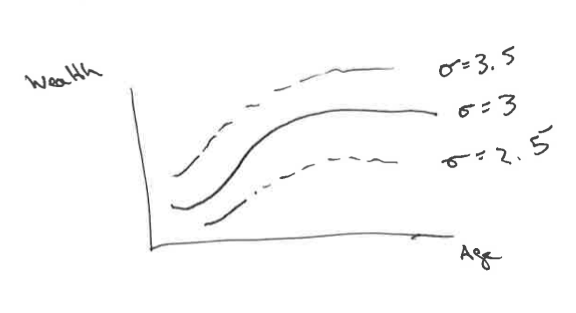
\includegraphics{pencildrawing.png}}}
\end{figure}


\end{document}

